\chapter{Audio Synthesizers}
\label{chapter:background}

\graphicspath{{./}{./figures/}{./figures/background/}}

In the context of audio, a synthesizer refers to a device that generates sound or music. Martin Russ provides a thorough overview of audio synthesis in his textbook, Sound Synthesis and Sampling \cite{russ2012sound}. Russ introduces the synthesizer as any device that generates sound,  even the human voice can be thought of as a synthesizer, however, sound synthesizers have become more broadly accepted as an electronic device that produces synthetic sounds. A synthesizer may do this through the playback and recombination of pre-existing audio material or through the generation and shaping of raw audio waveforms. There are numerous types of synthesis techniques that are capable of producing a huge variety of different sounds. 

%Broadly speaking, the sounds that a synthesizer generates can be categorized into two different classes: `imitative` or `synthetic`. Imitative sounds attempt to emulate a sound that exists in the natural world such as a physical musical instrument or a sound effect and synthetic sounds are those that have no relation to a sound in the physical world. The distinction between imitative and synthetic sounds is blurry and most sounds fall somewhere in the middle. Designing new sounds, whether they are imitative, synthetic, or somewhere in between, involves adjusting 

This chapter serves as background for audio synthesizers to provide context and motivation for research focused on improving their usability. Section \ref{section:synth-history} describes the evolution of synthesizers over time and provides historical context for some of the important developments in synthesizer technology that inform the research in this thesis. Section \ref{section:synth-anatomy} overviews some of the main components that a typical synthesizer comprises and introduces two of the most common types of synthesis. Section \ref{section:synth-programming} introduces the topic of synthesizer programming, including some of the challenges as well as opportunities for improvement. These challenges motivate the remainder of the research that is presented in this thesis. 

% Broadly speaking, these sounds can be categorized into two different classes: `imitative` or `synthetic`. Imitative sounds attempt to emulate a sound that exists in the natural world such as a physical musical instrument or a sound effect such as an explosion. Electric pianos are examples of imitative synthesizers. Synthetic sounds are those that have no relation to a sound in the physical world. The distinction between imitative and synthetic sounds is blurry and most sounds fall somewhere in the middle. For example, synth-brass sounds, which were a staple of synths such as Roland's popular Jupiter-8, are sounds that are based on an imitation of a brass sound but extend into the synthetic realm. 

% This is maybe a bit more like introduction material?
% Synthesizers have become ubiquitous in audio production and entire genres of music have been developed around their use. Bebe and Louis Barron produced the first electronic film score for the movie "Forbidden Planet" in 1955 using synthetic sounds. Since then the use of synthesizers for movies and video games has also become common-place.


\section{Evolution of Synthesizers}
\label{section:synth-history}

A brief history of the development and use of synthesizers is provided here for historical context. The full history of the topic is beyond the scope of this thesis and the interested reader is referred to some great textbooks that cover audio synthesizers and their history \cite{roads1980interview, mcguire2015musical, jenkins2019analog, russ2012sound}, which were used in the writing of this chapter.
\subsection{Analog Synthesizers}
Until the late 1950s all synthesizers were analog. Analog synthesizers are defined by their use of continuous-time signals, as opposed to digital systems which operate in discrete chunks of information and use discrete-time signals. Early analog synthesizers can be broken down into two broad categories: (1) sounds that are generated directly by electric circuits by oscillating vaccuum tubes, or (2) rotating or vibrating physical systems that are controlled by electronic sources \cite{roads1996computer}. The first, as well as the largest sound synthesizer ever built was developed in the early 1900s by Thaddeus Cahill. On September 26, 1906, an audience of 900 individuals came to view the massive electronic instrument called the Telharmonium that was capable of producing pure sinusoidal waves in at frequencies in integer ratios. Other early synthesizers include the Theremin, built by Leon Theremin in 1920, which produced a pure tone with a varying pitch and amplitude that was controlled by a performer moving their arms in relation to two antennas. Versions of the theremin have been used in popular music by musicians including The Beach Boys, Led Zeppelin, and The Rolling Stones.  The Ondes Martenot, developed in 1928 by Maurice Martenot and Ondes, had a similar sound to the theremin and also was one of the first synthesizers to include a piano-like keyboard interface.

In the 1960s two companies emerged on opposite sides of America and released synthesizers that have shaped the landscape of audio synthesis. Around 1964 Don Buchla, who lived in the San Francisco area, released the the Buchla 100 Series Modular Electronic Music System. At the same time in New York, Robert Moog released the R.A. Moog Modular System \cite{mcguire2015musical}. Both synthesizers were modular systems containing individual processing units called \textit{modules} that could be interconnected using patch cables. Connecting together synthesizer modules is known as creating a \textit{synth patch}, or simply a \textit{patch}. Both the Buchla and Moog systems introduced Voltage-Controlled Oscillators (VCOs) which create electronic waveforms at stable musical pitches, which can be controlled via an input signal called a control-voltage (CV). The Moog Modular System also featured a Voltage Controlled Filter (VCF) that was an early version of Moog's famous ladder filter design. This filter could resonate at a controllable frequency and was responsible for creating some of the most iconic synthesizer sounds that are still heard in contemporary music.

There were some important philosophical differences between Moog and Buchla Synthesizers that have lead to two different schools of thought: East Coast and West Coast synthesis. The development of the Buchla synthesizer by Don Buchla was guided by Morton Subotnick and other experimental composers working out the San Francisco Tape Music Center. Subotnick explicitly requested that the synthesizer was not controlled by a traditional keyboard interface as he was worried that it would trap him into created tonal music. Instead, Buchla synthesizers are controlled using a set of touch plates and sequencers. At the same time on the East coast Robert Moog was developing the Moog Modular and building a traditional keyboard interface to control the pitch of his VCOs. This feature, which allowed the Moog Modular Systems to be integrated more easily with Western music, was one of the reasons that Moog synthesizers became much more popular and commercially successful compared to Buchla. 

Another reason that Moog synthesizers were launched into the public eye is because of their use in recorded music. In 1968 Wendy Carlos used a Moog Modular synthesizer to orchestrate, perform, and record a selection of Johann Sebastian Bach pieces. The collection of music, called \textit{Switched On Bach}, went on to become the best selling classical recording of all time. Other musicians had created recreations of classical music pieces on synthesizers, but none had reached the same level as \textit{Switch On Bach}. Jenkins \cite{jenkins2019analog} credits the nature of the counterpoint in Bach's pieces as being particularly well suited to synthesizers, as well as Carlos' ability to design sounds that brought that performance alive, to the success of the release. Building on this success Carlos went on to score synthesized soundtracks for movies including Stanley Kubrick's \textit{A Clockwork Orange}. Another exceptional example of classical music recreated using Moog synthesizers worth mentioning is Japanese composer Isao Tomita's \textit{Snowflakes Are Dancing}, which was released in 1974. The use of synthesizers in music and film extends into almost all genres of music and was the cornerstone in the development of new genres including techno and other electronic music genres. For more information, see Mark Jenkins' overview of the use of synthesizers in throughout different genres of music in his book \textit{Analog Synthesizers: Understanding, Performing, Buying} \cite{jenkins2019analog}.

\subsection{Digital Synthesizers}
The first experiments with digital synthesis were conducted by Max Mathews on an IBM 704 computer in 1957 \cite{roads1980interview}. These experiments consisted of programming and synthesizing melodies using triangle waves, Mathew's program was able to accept the note pitch, amplitude, and duration. The Music III program was developed by Mathew's in 1960 and introduced an important concept called the \textit{unit generator}, which defined basic components of a synthesizer in programmatic units that a user was able to link together to create a full synthesizer architecture. Mathew's describes these concepts as being developed in parallel, but separately, to similar synthesis concepts (e.g. modular synthesizers) being developed in the analog world. He described this as "an advantage because a musician who knew who to patch together Moog synthesizer units would have a pretty good idea how to put together unit generators in the computer."

In 1973 John Chowning, a researcher at Stanford, released a landmark audio synthesis paper entitled on Frequency Modulation (FM) synthesis \cite{chowning1973synthesis}. The patent for FM synthesis was licensed to Yamaha who developed the Yamaha DX7 synthesizer using the technology, which was released in 1983 and became one of the best selling synthesizers of all time. One of the major benefits of FM synthesis is that it is able to produce complex audio waveforms at low computational cost. Additionally, the Yamaha DX7 was a fully polyphonic synthesizer, meaning that it was capable of producing multiple tones simultaneously (i.e. was able to play chords), whereas most analog synthesizers that were within the same time period were monophonic (only capable of playing one note at a time). The Yamaha DX7 was also incredibly difficult to program, although it came preloaded with a large selection of quality parameter settings, or presets, that allowed users to play the synth without have to learn how to program it.

As digital technology improved and computers became more powerful, new synthesis techniques such a sampling synthesis \cite{mcguire2015musical} and physical modelling \cite{jaffe1983extensions} emerged. Digital emulations of analog synthesizers, or virtual analog (VA) synthesis, also started to become popular in the 1990s. VA synthesizers attempt to express traditional analog synthesis methods in code as digital signal processing (DSP) algorithms. The development of more powerful computers also enabled recording workflows to be transferred into software and professional recording studios started to transition to digital with the release of Digidesign ProTools in the early 1990s. As software synthesis became more prevalent, many types of different software synthesizers emerged including VA software synthesis and a trend emerged of directly emulating analog equipment digitally, including the user interface. Skeumorphism describes computer user interfaces that attempt to directly mimic their real-world counterpoint, and has become extremely common in audio software, including synthesizers; user interface researchers have begun to question whether or not these skeumorphic interfaces enhance usability of not \cite{lindh2018beyond}.

\subsection{Audio Plugins}
In 1996 Steinberg\footnote{\url{https://www.steinberg.net}} released the Virtual Studio Technology (VST) interface, which allowed third-party software including audio effects to be integrated into host applications including DAWs. Because VSTs integrate with host applications, they are also called audio plug-ins. The second version of VST was released in 1999 which added support for the Musical Instrument Digital Interface (MIDI) \cite{rothstein1992midi}, a communication protocol enabling musical hardware and software to exchange information and control signals. The addition of MIDI to the VST interface opened the doors for VSTi, VST instruments, including software synthesizers. Other audio plug-in architectures have been developed in addition to VSTs, and popular ones include Apple's Audio Units (AU) and Avid's Avid Audio eXtension (AAX). Audio plug-ins have allowed software developers a method to create unique audio effects and synthesizers, and an industry dedicated to their development has blossomed over the last few decades. At the time of writing there are over 500 different synthesizer plug-ins available for purchase or for free on the KVR\footnote{\url{https://www.kvraudio.com/plugins/softsynth-virtual-instruments}} database of audio products.

\section{Anatomy of a Synthesizer}
\label{section:synth-anatomy}

Synthesizers can be viewed as comprising two major components: the \textbf{synthesis engine}, which is where sounds is generated, and a \textbf{control interface}, which allows a user to control the synthesis engine \cite{russ2012sound}. Audio synthesis can be a complex process, so there is generally a high-level of abstraction between the synthesis engine and the control interface. The role of the control interface is to present a conceptual model of the synthesizer to a user, which allows the user to express their ideas and modify the synthesis engine. The parameters on the control interface are mapped to components within the synthesis engine, often in non-linear ways. Figure \ref{fig:synth_abstraction} shows a diagram of the general components of a synthesizer and the control interface abstraction layer. The following sections provide more detail on each of the two major components of a synthesizer.

\begin{figure}[ht]
    \centering
    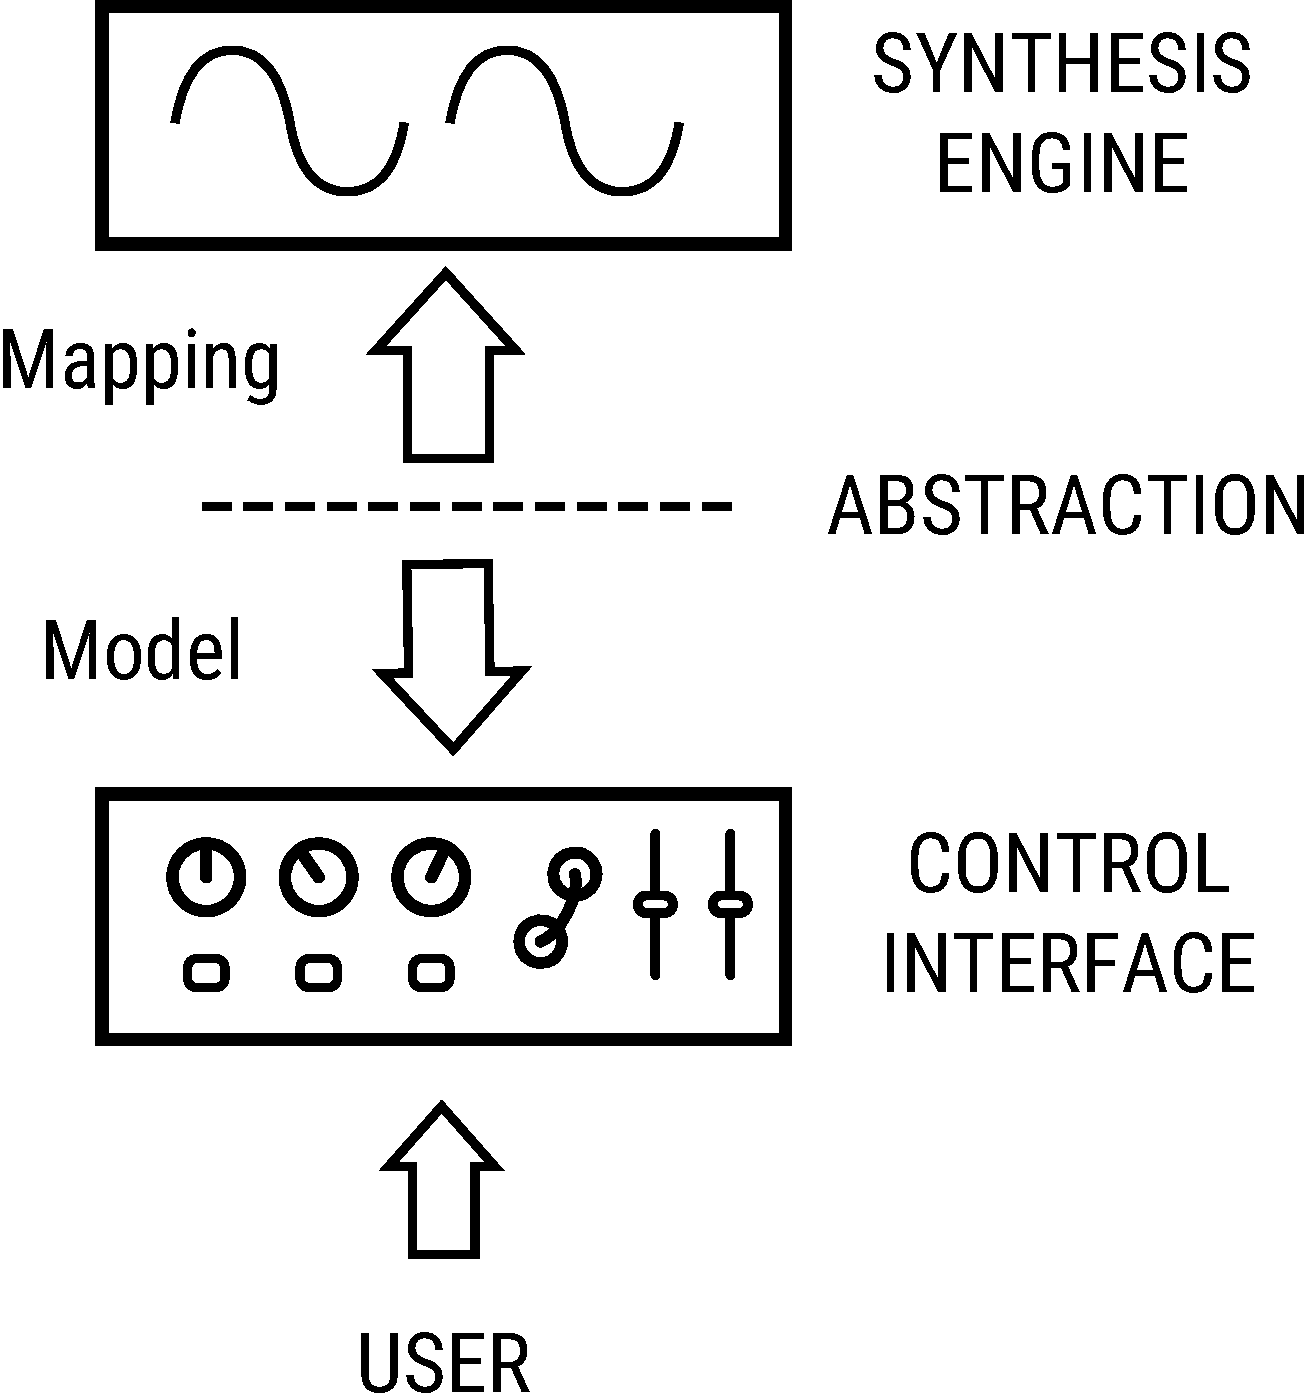
\includegraphics[width=0.4\textwidth]{figures/background/Synth Abstraction Model.pdf}
    \caption{Abstraction between the synthesis engine and control interface. A control interface on a synthesis is responsible for presenting a conceptual model of the underlying synthesis engine to a user. The parameters on the control interface are mapped back to the synthesis engine to modify audio generation.}
    \label{fig:synth_abstraction}
\end{figure}

\subsection{Synthesis Engine}
The synthesis engine is at the heart of sound generation in any synthesizer, whether it is an analog modular synth or a software audio plugin. Sam McGuire and Nathan Van der Rest provide an overview of the more popular synthesis methods in their book \textit{The Musical Art of Synthesis} \cite{mcguire2015musical}. These methods include: subtractive, sample-based, modulation (i.e. FM), additive, wavetable, granular, vector, and physically modelling. 

While the exact technique that each of these methods use may be different, there are some common components to synthesizers that exist in some form across many different techniques. It is useful to take a modular perspective when thinking about different synthesizer components, similar to the \textit{unit generator} concept introduced by Max Mathews \cite{roads1980interview}. From this perspective, different components of a synthesizer are broken down into functional units (modules) that can be interconnected in various ways to build up a full synthesizer. We can generalize modules as all producing some output signal as well as having an optional input signal. Modules may also have some parameters that can be mapped to a control interface for user control. We can broadly categorize the signals that are output by modules as either audio signals or control signals. Audio signals are generated by the synthesizer and ultimately are output as a sound. Control signals are used to modulate the parameters of other modules within a synthesizer. In some synthesizers audio signals can also be treated as control signals and be used to modulate parameters of other parameters at audio rate frequencies.

\subsubsection{Types of Modules}
We can categorize modules into two different types based on the type of signal they output: 1) \textbf{audio modules}, generate or process audio signals, and 2), \textbf{control modules}, generate or process control signals. Jenkins provides an overview of some of the different synthesizer modules from the perspective of an analog synthesizer \cite{jenkins2019analog}. In analog synthesis audio signals are commonly generated by voltage-controlled oscillators (VCOs). In a VCO the frequency of the oscillator is controlled by the voltage of an input control signal. While voltages only exist in analog circuits, the concept has been extended into digital synthesizers as well, with the digital equivalent of a VCO sometimes being referred to as a digitally controlled oscillator (DCO). Other common audio modules are voltage-controlled filters (VCFs), voltage-controlled amplifiers (VCAs), and Noise Sources; filters accept audio signals as input and attenuate or boost specific frequencies, VCAs are essentially an automated volume knobs, and noise sources generate different types of noise such as white noise.

Two common control modules are envelope generators (EGs) and low frequency oscillators (LFOs). Envelope generators are generally triggered in response to an event such a keyboard note being pressed. Once an EG has been initiated, it produces a control signal that evolves over time. The most common type of EG is an attack-decay-sustain-release (ADSR), which is triggered by a keyboard, rises to a peak level over a period over time defined by the attack, then falls to a level defined by the sustain over a period of time defined by the decay, stays at the sustain level until the keyboard press is released, and the finally falls back to zero over a period of time defined by the release. LFOs function the same as regular oscillators, but just at a low frequency, generally below 20 cycles per second. One common way that LFOs are used is to modulate the pitch on a VCO to create vibrato.

\subsubsection{Subtractive Synthesis}
Subtractive synthesis was one of the earliest methods explored and is the sound of the famous Moog synthesizers. It has been used on thousands of records, and is still a popular method. The basic idea behind subtractive synthesis is that the starting point is a harmonically rich waveform, generated by an oscillator, which is then sent through a chain of filters and other audio effects that shape the timbre of the waveform over time. [Insert a simple block diagram of a subtractive synth]. There are several types of waveforms that are generally available on a oscillator in a subtractive synthesizer, these are shown in figure X [insert a diagram of some of the common waveforms and their harmonics]. Each waveform has a unique set of harmonics. Harmonics refer to frequencies that are present in the sound that occur at integer frequency ratios to the fundamental frequency of the sound, which is associated to the perceived pitch of that sound. Sine waves are the simplest waveforms and only contain energy at the fundamental frequency. Noise generators produce energy at all frequencies and contain no fundamental frequency and are therefore inharmonic.

% Once a waveform has been generated it may be combined with other waveforms through a process called mixing. The average subtractive synthesizer has three oscillators \cite{russ2012sound} that are typically tuned to harmonically related frequencies. The next common stage in a subtractive synth signal path is an audio filter. As previously mentioned, one of the most famous synthesizer filters of all time is the Moog ladder filter \cite{moog1965voltage}, which is a resonant low pass/high-pass filter. Low pass filters allow low frequency sounds to pass through while attenuating frequencies above a certain threshold frequency, vice-versa for high-pass filters. The threshold frequency is usually controllable and can be modulated using other signals to create dynamic 'sweeping' sounds. After passing through the filter the signal passes through an amplitude gate, which acts as a volume knob that is controlled by an internal control signal envelope. The envelope 

\subsubsection{Frequency Modulation Synthesis}
FM synthesis was an another early method of synthesis that was developed during the origins of digital synthesis \cite{chowning1973synthesis}. FM synthesis engines are capable of producing a huge array of complex waveforms using a relatively simple structure, which makes them powerful, but more conceptually challenging to understand compared to subtractive methods. The basic unit of an FM synthesizer is referred to as an operator, which generally contains a single simple sine wave oscillator and an amplitude gate controlled by an envelope generator. The simplest FM synthesizer consists of two operators that are connected together so that one of the operators controls the frequency of the second operator. The operator that does the modulating is referred to as the \textit{modulator} and the operator that is modulated is referred to the \textit{carrier}. [Insert figure showing this arrangement.]


\subsection{Control Interfaces}
\label{sec:control_interfaces}

The control interface of a synthesizer allows a user to build up a conceptual model of the underlying synthesis engine so they can exert control over the sound being generated in an expressive way. Most synthesizers have interface components such a knobs and sliders that allow users to control the pitch, loudness, and timbre of a generated sound. Keyboard type interfaces and MIDI keyboard controllers provide a direct and easily understood method for controlling pitch, at least for those who are familiar with Western music traditions. Volume controls also provide a relatively direct method for controlling the loudness. The rest of the parameters on a synthesizer control interface are dedicated to controlling the timbre. Seago \cite{seago2004critical} conducted an analysis on synthesizer interfaces and describes three types:
\begin{enumerate}
    \item Parameter selection on a fixed architecture
    \item Architecture specification and configuration
    \item Direct specification of physical characteristics of sound
\end{enumerate}

% Add some images in here for some of the different interface types
Parameter selection interfaces present the user with an organization of parameters synthesizer modules that have been wired together in a fixed arrangement. Generally parameters are arranged in a hierarchical or structured way so as to represent the signal flow of the synthesizer architecture. These are the most common types of interfaces and were the type used on some of the early commercially successful units including the Moog Minimoog. A majority of software synthesizers emulate fixed architecture synthesizers and many software synthesizer also emulate the control interfaces of hardware interfaces. 

Architecture specification interfaces allow the user to wire together synthesizer modules in whatever way they want. Modular synthesizers are a good example of these types of interfaces. Software like VCV Rack\footnote{\url{https://vcvrack.com/}} provides emulations of Eurorack \cite{intellijel2019} hardware modular synthesizer modules in software. Cycling 74's Max/MSP\footnote{\url{https://cycling74.com/products/max}} and Native Instrument's Reaktor\footnote{\url{https://www.native-instruments.com/en/products/komplete/synths/reaktor-6/}} are other examples of architecture specification interfaces implemented in software.

Direct specification interfaces make an attempt to allow the user to interact with the sound object itself, as opposed to interacting with a conceptual model of a sound engine. A visual representation of sonic material is presented, typically as the time-domain waveform or a representation of the frequencies. Users are able to draw-in and shape the output sound through this visual interface. This type of interaction can be challenging due to the complex relationship between the visual representation of a sound and its perceptual quality. Some software synthesizes provide users a form of direct specification within a larger more traditional architecture: Xfer Records Serum\footnote{\url{https://xferrecords.com/products/serum}} allows users to draw in custom waveforms for wavetables and Izotope Iris\footnote{\url{https://www.izotope.com/en/products/iris.html}} has a visual interface to draw in the frequencies of a spectral filter, shown in \ref{fig:izotope_iris}. \cite{knees2016searching} -- mental images. (this maybe goes into the automatic synthesizer programming section on academic work.

\begin{figure}[ht]
    \centering
    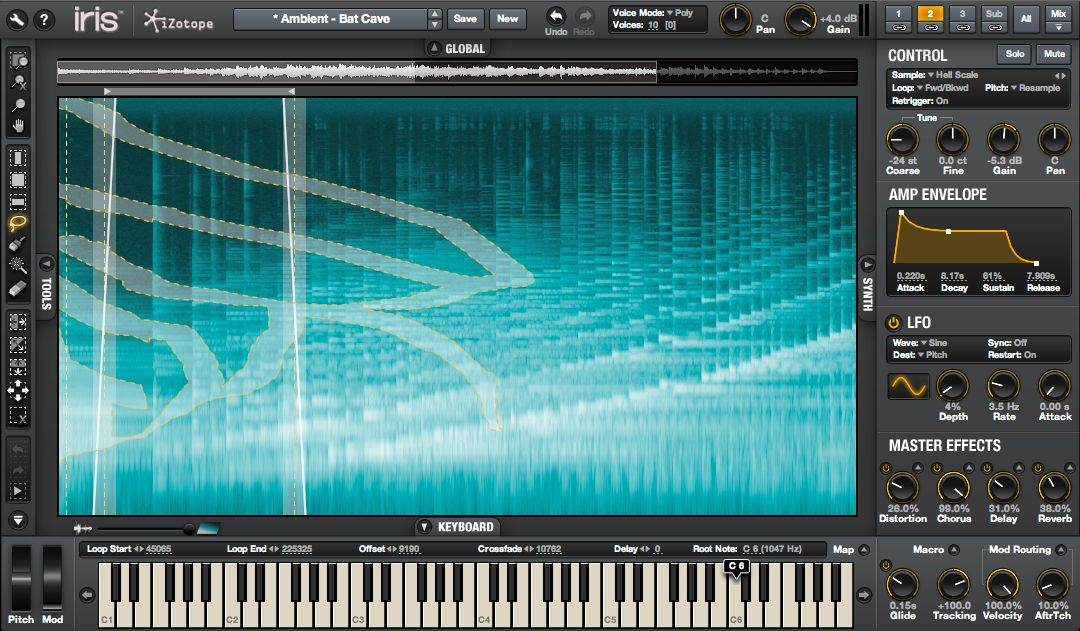
\includegraphics[width=0.80\textwidth]{figures/background/izotope_iris.jpg}
    \caption{Izotope Iris. A sample-playback synthesizer plugin with a visual interface that allows users to draw in frequencies.}
    \label{fig:izotope_iris}
\end{figure}

\subsubsection{Skeumorphism}
A common trend in synthesizer control interface design worth mentioning is the use of use skeumorphism. Skeumorphmic interfaces are computer user interfaces that attempt to directly mimic their real-world counterpoint. Development of these types of interfaces have become extremly common in audio, partly due to nostalgia and fetishization of analog audio gear [cite me!]. Many software synthesizer plug-ins implement these interfaces,despite the ability for developers to create more nuanced and flexible user interfaces using computer graphic user interfaces (GUIs). For example [include an image of minimoogs both in hardware and in software]. Researchers have begun to question whether or not these skeumorphic interfaces enhance or hinder usability of audio software \cite{lindh2018beyond}. 

Not all software synthesizers utilize skeumorphism and many have introduced new structured methods for organizing the UI onto different pages or subsections that would not be possible on a physical device. One aspect of all control interfaces that is almost universal between hardware and software synthesizers is the use of "knobs", "faders", and other physical controls as parameters. Even though turning a knob with a mouse is quite an awkward interaction, this paradigm is pervasive.

% Not so sure about this section.
% The nature of the control interface is guided by the synthesis method being used by the engine. Synthesis methods like subtractive synthesis which involve a clear linear signal flow that starts with a complex waveform that is progressively shaped can lead to a more simple conceptual model. Moog synthesizers are examples of subtractive synthesizers that have clear control interface that maps to the synthesis engine. More complex synthesis methods such as Frequency Modulation (FM) synthesis are more challenging to create clear control maps for. Interestingly, the most commercially successful synthesizer, the Yamaha DX7, had a notoriously difficult control interface, although shipped with an extensive high-quality set of factory presets (pre-defined control interface parameter settings).


% Bounce this out to another section I think. This could sit in creativity support potentially?
% \subsubsection{Neural Synthesis}
%One area of new development in audio synthesis is in methods that are leveraging advancements from the field of deep learning [deep learning cite], an area of audio synthesis that is explored in this thesis.  
% In contrast to traditional synthesis, neural synthesizers generate audio using large-scale machine learning architectures with millions of parameters \cite{engel2017neural}. Differentiable digital signal processing \cite{engel2020ddsp} bridged the gap between traditional DSP synthesizers with the expressiveness of neural networks, exploring a harmonic model-based approach, using a more compact architecture with 100K parameters.
% One benefit of synthesized audio is that the underlying factors of variation ({\em i.e.}~the parameters) are known.

% % GANs for synthesis
% In this work, we use Generative Adversarial Networks (GANs) \cite{goodfellow2014generative} to generate new instrumental audio from a dataset of existing material. GANs have the potential to be used to generate new sounds on the fly. This would dramatically alleviate both the problem of having to pore through giant sound libraries, and the problem with having to only use one sample repeatedly. In addition, the explosion of new sounds which could potentially be produced by GANs would vastly reduce recording costs by designers of sound libraries.

% This research avenue is to a certain degree untapped: GANs have been successfully applied to the generation and manipulation of images, however, relatively little work has been focused on the audio domain. Research related to the specific work proposed here was presented by \cite{donahue2018adversarial}  and \cite{engel2018gansynth}.
%\cite{ccakir2018musical} - not totally sure what this is about, I think it is generative though.

\section{Synthesizer Programming}
\label{section:synth-programming}

When trying to get a particular sound out of a synthesizer, users generally have two options: they can try to build up the sound from scratch by adjusting parameters, or they can hope that someone else has gone through that process for them and search through a database of pesets to find a sound that fits their criteria. Many users use a combination of these two approaches and use a preset as a starting point and adjust parameters to tune the sound \cite{krekovic2019insights}. The act of programming a synthesizer refers to the process of manually adjusting parameters, whether from scratch or using a preset as a starting point. Synthesizer programming is not an easy task, requiring strong technical understanding of the particular synthesizer and ability to express creative ideas through the control interface. Carlos and Tomita were masters at programming rich sounds that worked perfectly for their music, and is one of the reasons their work achieved critical acclaim \cite{jenkins2019analog}. Specific techniques for programming synthesizers have lead to the creation of sounds that define genres of music, especially electronic music, such as the "wobble bass" sound characteristic of Dubstep and or "squelchy synth lines" of Acid House tracks. 

The growing accessibility of hardware and software synthesizers has resulted in an unprecedented number of audio practitioners and hobbyists purchasing and desiring to learn how to program synthesizers. This is reinforced by the fact that there are currently 147 different videos courses available for sale on the Groove3 online education platform teaching synthesizer programming for various virtual instruments\footnote{\url{https://www.groove3.com/browse}}. In a recent study, users reported on the challenges associated with learning to user various synthesizers and a expressed a desire for improved user interaction methods \cite{krekovic2019insights}. The growth in interest in amongst musicians to learn to program synthesizers, along with desires for more intuitive ways to work with them points to the need for additional research in this area. This serves as motivation for the research conducted in this thesis. The remainder of this section expands on the challenges associated with synthesizer program to further develop the research motivation, and then finishes with some opportunities for future work that have been identified through user studies and serve as a guide through this work.

\subsection{Challenges}
\textbf{[Incomplete]}

The need for improved methods for learning how to work with and program synthesizers was first identified in published work in the later 1970s by James Justice \cite{justice1979analytic}. Justice describes the difficulties he faced in trying to answer his students questions about how to program specific sounds into an FM synthesizer. 
- Keep this simple. 
- Talk about the Pardo description of the different conceptual models

\cite{ashley1986knowledge} provides a good overview of some of the challenges associated with programming an FM synthesizer.

In the previous section on synthesizer control interfaces, \S\ref{sec:control_interfaces}, three different dimensions of sound were introduced: pitch, loudness, and timbre. Pitch and loudness are uni-dimensional and have relatively simple mappings to parameters \cite{seago2004critical}. The remaining parameters on a synthesizer, which is the vast majority of them, are used to specify the timbre of the resulting sound. This means that the primary task of programming a synthesizer is using a control interface to design the timbre of a sound. 

But what is timbre? The ANSI definition describes it as the attribute of auditory sensation that allows it to be distinguished from other sounds at the same pitch and loudness \cite{american1973american}. This definition doesn't tell us very much about what timbre is, as opposed to what it is not. Understanding precisely what musical timbre \textit{is} has presented itself as challenging problem \cite{krumhansl1989musical} and significant research has been conducted to try to answer this \cite{McAdams2019}. The spectrotemporal conception of timbre [cite Risset] describes timbre as a series of time-varying spectrums. Building on this, Grey introduced the concept of \textit{Timbre Space} \cite{grey1977multidimensional} as a multidimensional representation of timbre. Risset and Wessel explore timbre in the context of sound synthesis and emphasize the importance of considering the evolution of frequencies over time \cite{risset1999exploration}. 

- What can we draw from this: Programming a synthesizer is specifying how a spectrum evolves over time. It is impractical to do this directly considering the number of parameter values that would need to be set and the values themselves are not easily subjectively interpretable. Different synthesis techniques provide methods for accessing vast regions of the space possible timbres using a more compact set of parameters. 

The complexity of defining what timbre is and how we can accurately represent it highlights one of the challenges of synthesizer programming: users are tasked with navigating a complex multidimensional perceptual space that doesn't have clearly defined boundaries or axes. 

Synthesizer control interfaces provide the means for navigating this space. Most manufacturers avoid venturing into the vague territory of providing perceptually motivated controls and instead allow the underlying synthesis engine to dictate the design \cite{seago2004critical}. As a result, timbre control is mostly specified by a large number of numerical parameters that are unique to the synthesis technique \cite{ethington1994seawave}. Allan Seago describes some of the challenges in programming synthesizers based on various synthesis techniques \cite{seago2013new}:

\begin{quote}
    Some [synthesis techniques], like subtractive synthesis, offer controllers which are broadly intuitive, in that changes to the parameter values produce a proportional and predictable change in the generated sound. Other methods, however, are less easily understood. FM synthesis, for example, is a synthesis method that may be viewed as essentially an exploration of a mathematical expression, but whose parameters have little to do with real-world sound production mechanisms, or with perceived attributes of sound.
\end{quote}

Both Wendy Carlos and Isao Tomita were both masters at programming synthesizers. They learned the connection between the parameters of the synthesizers and how to interconnect modules to create the rich timbres that made their music so special. This involved developing a deep understanding of the technical details of the synthesis engine, how the parameters affected synthesis, and how to proficiently navigate the timbre space of their synthesizers. A recent study conducted by Gordan Krekevi\'{c} sought to elucidate how a more general population of synthesizer users \cite{krekovic2019insights}. 122 individuals participated in that study, which consisted of an online survey with questions regarding their experience with synthesizers. A majority of users were very experienced with synthesizers, 71\% had ten or more years of experience, and only 2.7\% were novice users, having less then a few months of experience. Additionally, a majority of users had some formal training as musicians, although having formal musical training was only a weak indicator of experience using synthesizers. When asked about how they engaged with their synthesizers users claimed that they would most often program sounds from scratch or modify a preset as opposed to using a preset with no modification. Interestingly, there was no correlation with experience or level of music education; all users, regardless of their background experience, most often engaged in the manually tweaking parameters of their synthesizers to create sounds. 

Krekov\'{c} identified four impediments to manually programming a synthesizer:
\begin{enumerate}
    \item it can be time consuming,
    \item it can be a distraction from focusing on music,
    \item it can be difficult and non-intuitive to learn to use a particular instrument,
    \item it rarely leads to desirable results.
\end{enumerate}

Most participants agreed with statements 1-3 and disagreed with statement 4, however, participants with less experience were more likely to agree with statement 4 and participants who more often programmed from scratch were less likely to agree. This indicates that users with more experience programming synthesizers more often felt that they were able to achieve desirable results. When given the opportunity to write about their experiences in a more open-ended manor participants generally reported on difficulties with user-interfaces, learning specific synthesizers, limited features, and the creative process. One participants' comments highlight some of the challenges and commitment associated with learning to use synthesizer.

\begin{quote}
    Different sorts of synthesis require different background knowledge, most of which have steep learning curves that are at least partially exclusive. In other words, there is an enormous investment of time to deeply learn how the different forms of synthesis work. This learning is a prerequisite to effective use of synthesizers.
\end{quote}

\subsection{Opportunities}
\textbf{[Incomplete]}

Considering that well over half of the participants in Krekovi\'{c}'s study had over ten years of experience, the results highlight the degree of difficulty associated with programming synthesizers and the opportunity for improvements. Finding alternative and assistive methods for synthesizer programming has been an active field of study for over 40 years and will be reviewed in detail in the following chapter. Based on a review of some of the methods from previous research, Krekovi\'{c} selected four different methods and asked participants to rate the perceived helpfulness of each system. The systems proposed were: 1) a system that generates random presets within a category, 2) a user provides a description of a the desired sound and a preset is generated for them, 3) a user provides an example sound and the system generates a presets to sound similar, and 4) more intuitive interactive user interface. Participants thought that proposed systems 3 and 4 would be helpful and systems 1 and 2 would be slightly helpful. 

Due to the limited number of novices included the study, it is challenging to to say with certainty how these results would generalize to users in that category, and this would be a good area for future work. However, based on the results that showed a correlation between experience and satisfaction with results of programming, there is likely a good opportunity to improve the experience of novice users.

%\subsection{Enjoyment}
%When conducting a critical analysis on the usability of synthesizers and the affect that has on synthesizer programming, it is easy to take on the perspective that it is a strictly negative trait that synthesizers are challenging to use and that is something that must be improved. There is, however, some indication that users enjoy the complexity of synthesizer interfaces and the challenge that provides in their programming. This is illustrated by the recent resurgence in hardware modular synthesizers \cite{bates2021interface}. Modular synthesizers are more complicated and time-consuming to use than software synthesizers for a number of number of reasons, and are more likely to lead to unsatisfactory results, yet the demand for them has shot up in recent years. This points to realization that programming a synthesizer, despite it being challenging and time-consuming, is an enjoyable experience and something worth doing regardless of the quality of the final result. Results from Krekovi\'{c}'s study point to this conclusion as well, despite the fact that participants agreed with three out of four of the impediments, they still chose to manually program more often than not, and most had for many years. This conclusion could of course be drawn based on survivor bias, the users who participated in the study hadn't given up with synthesizer programming in the face of the challenges; they either enjoyed it enough, or had another good reason, to keep going despite the impediments. How many potential synthesizer users are not represented because they never made it past the initial learning curve? While it is arguable whether using a musical instrument should be easy \cite{mcdermott2013should}, and that long term enjoyment may depend on the existence of challenges and idiosyncrasies, there is most certainly an opportunity to improve and support the enjoyment of synthesizer programming at all stages of a users' process.


% - \cite{bates2021interface} - looks at interfaces of modular synthesizers (maybe better in control interfaces?) 
% - \cite{d2016interface} interface of software synthesizers and smart phones?

% A skilled sound designer is able to interact with the control interface and craft sounds to fit the needs of their creative project. This process is referred to as programming a synthesizer. 

% Both Carlos and Tomita excelled at patching synthesizer modules together and tuning the parameters of individual modules to create new sounds to orchestrate their performances. This process ... it's art! Blah blah blah. But also these folks are artists and virtuosos.

% - Challenges identified in \cite{ethington1994seawave}: Timbre is most commonly specified by a large collection of numerical parameters peculiar to a particular synthesis technique."
% - Challenges with synthesizer programming UI design: \cite{seago2013new}. -- "Some, like subtractive synthesis, offer controllers which are broadly intuitive, in that changes to the parameter values produce a proportional and predictable change in the generated sound. Other methods, however, are less easily understood. FM synthesis, for example, is a synthesis method that may be viewed as essentially an exploration of a mathematical expression, but whose parameters have little to do with real-world sound production mechanisms, or with perceived attributes of sound." -- There are some other really good bits about navigating the timbre space and non-linearities.
% - \cite{seago2004critical} Thus, under most current systems, the user is obliged to express directives for sound specification in system terminology, rather than in language derived from the user domain. Three types of synthesizer interfaces: parameter selection in a fixed architecture, architecture specification and configuration, and direct specification of physical characteristics of sound.
% - Context on synthesizer programming \cite{jenkins2019analog}
% - Russ describes the programming component intrinsically creative.
% - When we talk about programming synthesizers we are referring to the task of selecting parameter settings for a synthesizer in order to achieve a desired sound
